\section{Angular obstructions and the final contradiction}
\label{sec:angular}

We now show that none of the three cycle lengths supplied by
Proposition~\ref{prop:interface-cycle} is possible.  Fix its common
center \(x\), cyclically index the cycle labels by \(j\), and let
edge \(j\) join labels \(j\) and \(j+1\).  Write \(K_j\) for its
continuum and \(v_j\) for its limiting unit direction.  Thus there
are points
\[
 q_{j,n}=x+r_{j,n}w_{j,n}\in K_j,\qquad
 r_{j,n}>0,\quad r_{j,n}\longrightarrow0,\quad
 w_{j,n}\in S,\quad w_{j,n}\longrightarrow v_j.
\]
The rays used below record only these selected limiting directions
\(v_j\); no straight ray segment is assumed to lie in \(K_j\).
All palettes in this section are at this fixed center.  As before,
\(R\) rotates by \(\kappa=\pi/3\), and \(J\) by \(\pi/2\).

\subsection{Restrictions on the two sides of the unit circle}

The one-sided strips below are a counterpart of the complementary-color
strips in \citet[Proposition~9]{SokolovVoronov2025}. Related circle and
complementary-arc arguments also occur in
\citet[Sections~3--5]{Voronov2025Interval}, for a positive interval of
forbidden distances. We use only the single forbidden distance one;
the input is the exclusion continua just extracted.

Let \(\mathcal B\subset S\) be the finite, antipodally symmetric
set of directions perpendicular to at least one \(v_j\).
At \(e\notin\mathcal B\), give edge \(j\) sign \(+\) or \(-\)
according as \(e\cdot v_j\) is positive or negative.  Let \(O(e)\)
be the set of labels remaining after the endpoints of every positive
edge are removed, and let \(I(e)\) be the set remaining after the
endpoints of every negative edge are removed.  Labels outside the
cycle belong to both sets.

\begin{lemma}[One-sided strip restrictions]\label{lem:angular-strips}
Both \(O(e)\) and \(I(e)\) are nonempty for every
\(e\notin\mathcal B\).  On an angular neighborhood of \(e\), an
open strip just outside radius one uses only \(O(e)\), and an open
strip just inside radius one uses only \(I(e)\), in both cases up
to plane-null sets.  Moreover,
\begin{equation}\label{eq:source-25}
 P_x(e)\cap O(e)\ne\varnothing,
 \qquad P_x(e)\cap I(e)\ne\varnothing
 \quad\text{for almost every }e\in S\setminus\mathcal B.
\end{equation}
\end{lemma}

\begin{proof}
For a positive edge sign, the identity
\[
 \abs{x+e-q_{j,n}}^2
 =1+r_{j,n}^2-2r_{j,n}(e\cdot w_{j,n})
\]
is strictly less than one for some sufficiently large fixed \(n\).
By continuity, the strict inequality holds when \(e\) varies in
a small angular neighborhood and its radius increases slightly
above one.  Such points have distance greater than one from
\(x\in K_j\) and less than one from \(q_{j,n}\in K_j\); they lie
in \(\Delta(K_j)\).  Proposition~\ref{prop:interface-cycle} excludes both
endpoint essential supports there.  If the sign is negative,
the displayed distance is greater than one for large \(n\), and
the same argument at radii slightly below one gives the inner
strip.  There are finitely many edges, so the angular neighborhoods
and positive radial widths can be intersected.  An empty allowed
set would exclude every color from a nonempty open strip, contrary
to the measurable partition.

Cover \(S\setminus\mathcal B\) by countably many smaller arcs
on each of which all signs are constant and both strip restrictions
hold with positive widths.  For each such arc, polar-coordinate
Fubini gives the relevant restriction almost everywhere angularly
for almost every radius in its permitted interval.  Impose no
condition from that arc outside its permitted interval; its failures
then exclude only a null set from the whole radial half-line.
Intersect these countably many full-measure radial conditions with the
full-measure condition of typical sampling at center \(x\).
Choose radii from this intersection tending to one from above.
For each fixed arc the outer restriction eventually holds along
the entire sequence.  A weak-* subsequential trace in
\(\mathcal W_x\) has zero coordinates for the excluded labels
on that arc.  Its coordinates sum to one, and its positive
coordinates belong to \(P_x\) almost everywhere, so it supplies
an outer allowed palette member.  Countably many arcs suffice.
A separate sequence tending to one from below proves the inner
assertion.  The two sides need not use the same trace.
\end{proof}

\subsection{Exclusion of a five-cycle}

\begin{proposition}\label{prop:angular-five}
The extracted interface cycle cannot have length five.
\end{proposition}

\begin{proof}
Index its five labels modulo five.  A label belongs to \(I(e)\)
exactly when its two incident signs are positive, and to \(O(e)\)
exactly when both are negative.  Their nonemptiness requires a
pair of consecutive signs of each kind.  If there were two or
more runs of each kind, the two required runs of length at least
two and the other two nonempty runs would occupy at least six
positions.  Thus the five signs consist of one positive run and
one negative run, of lengths two and three in some order.

The allowed sets are the internal vertices of these runs, of
sizes one and two.  They are disjoint.  The palette size bound
\eqref{eq:source-13} and \eqref{eq:source-25} imply that almost
every palette is a pair, containing one vertex from each allowed
set.  Put \(D_i=\{i,i+2\}\).  After a cyclic relabeling, the
length-two run occupies edges \(0,1\), with middle vertex \(1\),
and the length-three run occupies edges \(2,3,4\), with internal
vertices \(3,4\).  The two possible palettes are therefore
\(D_1=\{1,3\}\) and \(D_4=\{4,1\}\), whose indices differ by
two modulo five.  Reversing every sign interchanges the two
allowed sets and preserves these options.  Consequently the
palette options at antipodal directions are identical.

Choose a direction on a full six-position \(R\)-orbit for which
all the preceding almost-everywhere assertions and
\eqref{eq:source-12} hold.  Write \(p_j\in\Z/5\Z\) for the
index of its palette \(D_{p_j}\) at \(R^je\).  Two diagonals
\(D_a,D_b\) are disjoint exactly when \(b-a=\pm1\) modulo five.
Thus successive indices make steps \(\varepsilon_j\in\{1,-1\}\),
including the closing step from position five to position zero.
For antipodal positions \(j,j+3\), the common two-element option
set allows index difference only \(0\) or \(\pm2\).
But the possible sums of three steps are \(-3,-1,1,3\); none
is zero modulo five, and a sum is \(\pm2\) modulo five only if
all three steps have the same sign.  Every consecutive triple
of steps must therefore be constant.  Overlapping triples force
all six signs to agree, whereas six equal steps do not close
modulo five.  This is the desired contradiction.
\end{proof}

\subsection{Four-cycle words and projective ray geometry}

Suppose next that the cycle labels are \(0,1,2,3\), with outsider
\(X\), and put \(U=\{0,2\}\), \(V=\{1,3\}\).
If \(X\notin P_x(e)\), the two requirements in
\eqref{eq:source-25} force a consecutive pair of positive signs
and a consecutive pair of negative signs.  Hence the four signs
are a cyclic run of two of each sign, which we call a
\emph{split}.  The two allowed sets, after removing \(X\), are
the opposite middle vertices of the runs.  They determine a
diagonal \(d(e)\in\{U,V\}\), and \(d(-e)=d(e)\).

Define the effective state \(p(e)\) to be \(X\) whenever
\(X\in P_x(e)\), and otherwise to be the forced diagonal
\(d(e)\).  The group represented by this state is contained
in the palette: it is the singleton \(\{X\}\) in the first
case and the entire diagonal in the second.  Consequently,
\begin{equation}\label{eq:source-26}
 p(e)\ne p(Re),\qquad
 p(e)=p(-e)\ \text{if both states are different from }X,
 \quad\text{almost everywhere}.
\end{equation}
If a diagonal occurs only on a null set, the remaining
singleton-versus-pair state system contradicts
Lemma~\ref{lem:transitions-two-state}; a single remaining state
already contradicts the first assertion in \eqref{eq:source-26}.
We may therefore suppose that both diagonal states have positive
angular measure.

For a nonparallel pair of density-one directions of the \(U\)
and \(V\) state sets, the density conclusion of
Lemma~\ref{lem:palette-transfer} excludes all four cycle labels
at their sum with \(x\).  That sum has density one of \(X\).
Lemma~\ref{lem:transitions-strict-separation} now applies to these
three represented groups.  If \(F_U,F_V\) denote the compact
angular essential supports of the diagonal state sets, then
\[
 F_D\cap RF_D=\varnothing\qquad(D=U,V).
\]
The same holds for \(R^{-1}\).  Compactness provides a common
positive angular separation margin.

Choose a dense conull set \(G\) of angular parameters, invariant
under addition of \(\kappa\), on which all six orbit positions
avoid \(\mathcal B\), satisfy the state rules, and belong to
\(F_U\) or \(F_V\) whenever the respective state occurs.  Define
\[
 w(t)_j=p(e^{i(t+j\kappa)}),\qquad j\in\Z/6\Z,
 \quad t\in G.
\]
There exists \(\eta>0\) such that whenever \(t,t'\in G\)
have circular angular distance less than \(\eta\), a diagonal
at any position of \(w(t)\) cannot equal a diagonal at an
adjacent position of \(w(t')\).  Indeed, such equality would
give points of the same compact essential support at angular
distance less than the margin from an \(R\)- or \(R^{-1}\)-pair.
We refer to this as the cross-word restriction.

\begin{lemma}[Six-position word alternatives]\label{lem:angular-words}
Every word \(w(t)\) contains \(X\), and all its \(X\) positions
have the same parity.  Every direction outside \(\mathcal B\)
is split.
\end{lemma}

\begin{proof}
A word without \(X\) alternates \(U,V\) by adjacent inequality,
contradicting the antipodal equality in \eqref{eq:source-26}.
Suppose that \(X\) occurs on both parities.  Any pair of its
opposite-parity positions must be antipodal, since otherwise
they are adjacent on the six-cycle.  There are exactly two
such occurrences: fixing one on each parity prevents any
additional occurrence on either parity.  Cyclically shift
them to positions zero and three.  Positions one and two
are distinct non-\(X\) states, and their antipodes four and
five have the same respective values.  Thus the word is a
three-periodic permutation of \(X,U,V\).

Such a word is isolated under the cross-word restriction.
In any compatible nearby word, each of its positions zero
and three has neighbors \(U,V\) in the original word; it
must therefore be \(X\).  The remaining four positions are
non-\(X\) by their own adjacent inequality.  If the original
positions one and two are \(U,V\), the cross-word restrictions
against position two and position one, respectively, force
the new positions one and two to be \(U,V\); the other block
is forced in the same way.  Hence the new word is identical.

Any two points of a dense subset of the circle can be joined
by a finite chain within that subset whose steps have angular
distance less than \(\eta\): subdivide a connecting arc into
steps smaller than \(\eta/3\) and approximate its intermediate
vertices by points of the dense set.  Isolation would therefore
propagate this word throughout \(G\).  But
\(w(t+\kappa)_j=w(t)_{j+1}\), and a three-periodic permutation
word is not equal to its one-position shift.  Since \(G\) is
shift invariant, this is impossible.

It follows that the nonempty set of \(X\) positions has a
unique parity, denoted \(h(t)\in\Z/2\Z\).  The three positions
of the other parity are non-\(X\), hence split.  They contain
one representative from each antipodal pair of positions.
Since splitting is antipodally invariant, all six positions
are split.  In particular almost every direction is split.
Signs are locally constant outside the finite set \(\mathcal B\).
A nonsplit direction there would have a nonsplit open
neighborhood of positive measure, which is impossible.
\end{proof}

\begin{lemma}[Geometry of four split rays]\label{lem:angular-four-rays}
Under the conclusions of Lemma~\ref{lem:angular-words}, the four
rays consist of two distinct antipodal pairs.  Opposite directions
occupy opposite edge positions.  On the projective angular circle
of circumference \(\pi\), the forced diagonal \(d\) equals \(U\)
on one open arc and \(V\) on its complementary open arc.  One
of these arcs has length at most \(\pi/2\).
\end{lemma}

\begin{proof}
Every generic open semicircle \(\{v:e\cdot v>0\}\) selects
exactly two rays, counted with multiplicity, and the selected
edge positions are adjacent.  At a boundary perpendicular to
one unoriented ray line, cross the boundary without crossing
any other such boundary.  The selected multiplicity on that
line changes from the number of its rays in one direction
to the number in the opposite direction; all other selections
stay fixed.  Equality of the total count before and after
shows that these two multiplicities coincide.  Thus all rays
are antipodally paired.

If only one unoriented line occurs, it has two rays in each
direction.  The selected edge positions are a fixed adjacent
pair or its complement.  These two split patterns give the
same diagonal.  The other diagonal could not occur on a set
of positive measure, contrary to our assumption.  There are
therefore two distinct lines, with one ray in each of their
two directions.

A specified ray on one line can be positive simultaneously
with either ray on the other line: the corresponding two
nonopposite unit directions fit in an open semicircle.
Its edge position is consequently adjacent to both positions
from the other line.  In a four-cycle the remaining position
is its opposite, so its antipodal ray occupies the opposite
edge position.  This applies to both lines.

Modulo antipodes, the two perpendicular boundaries divide
the angular circle into two open arcs.  The signs, up to
global reversal, are constant on each arc.  Crossing a
boundary replaces one selected edge by its opposite while
keeping the selected edge from the other line.  The two
middle vertices of the resulting split are the other
diagonal.  Thus the forced diagonal takes the two different
values on the two arcs.  Their lengths sum to \(\pi\), which
proves the last assertion.
\end{proof}

\begin{proposition}\label{prop:angular-four}
The extracted interface cycle cannot have length four.
\end{proposition}

\begin{proof}
Suppose \(t,t'\in G\) are less than \(\eta\) apart and
\(h(t)\ne h(t')\).  Select the three positions opposite to
the \(X\) parity in \(w(t)\), and the other three positions
opposite to the \(X\) parity in \(w(t')\).  All selected
states are diagonals; around the six positions they alternate
between the two words.  Cross-word adjacent states differ.
Since only \(U,V\) are available, all three selected entries
of the first word have one diagonal value, and all three
of the second have the other value.

For either word the three selected directions, projected
modulo antipodes, are spaced equally by \(\kappa\).  Each
is a non-\(X\) direction, so the forced diagonal there is
its selected value.  Both of the open diagonal arcs in
Lemma~\ref{lem:angular-four-rays} would therefore contain
three equally spaced projective positions.  An open arc
containing such three positions has length greater than
\(2\pi/3\): its closed complementary arc avoids the three
points, so lies strictly inside one of the three gaps and
has length less than \(\pi/3\).  This contradicts
the diagonal arc of length at most \(\pi/2\).

Thus \(h\) agrees at all sufficiently close points of \(G\).
The dense-set chain argument from
Lemma~\ref{lem:angular-words} makes it constant on \(G\).
Yet shifting by \(\kappa\) shifts every word by one position
and reverses this parity.  The shift invariance of \(G\)
gives a contradiction.
\end{proof}

\subsection{Triangle interfaces force alternating sectors}

It remains to consider a triangle cycle.  Call its labels the
\emph{triangle labels}, and write \(X,Y\) for the outsiders.
At every \(e\notin\mathcal B\), two of the three edge signs
agree.  Those two edges cover all three triangle labels.
Lemma~\ref{lem:angular-strips} therefore provides an open
strip on an angular neighborhood of \(e\), approaching radius
one from one side, which uses only \(X,Y\) almost everywhere.
Equation~\eqref{eq:source-25} gives an outsider in \(P_x(e)\)
almost everywhere.  There cannot be two outsiders in such
a palette, since \eqref{eq:source-12} would leave no outsider
at \(Re\).  We obtain a measurable binary state
\[
 s(e)\in\{X,Y\},\qquad s(Re)\ne s(e)
 \quad\text{almost everywhere}.
\]

The use of two complementary colors near a unit circle has a
predecessor in Townsend's annulus argument
\citep[Theorems~1 and~4]{Townsend2005}; here the restrictions hold
almost everywhere and need not form an annulus.  The next lemma
extracts local constancy directly from the open strips.

\begin{lemma}[Local binary rigidity]\label{lem:angular-binary-local}
If \(e_0,Re_0\notin\mathcal B\), then \(s\) is almost
everywhere constant on an angular neighborhood of \(e_0\).
\end{lemma}

\begin{proof}
Let \(\mathcal U,\mathcal V\) be the open strips restricted
to \(X,Y\) near \(e_0,Re_0\), respectively.  Each approaches
radius one from its prescribed side, and these sides may
differ.  Put \(z_0=x+e_0\).  There are two nonparallel unit
directions \(v'_1,v'_2\) such that
\(z_0+v'_j\in\mathcal V\).  To verify this, rotate so
\(e_0=1\) and consider
\[
 F(r,\theta)=\abs{r e^{i\theta}-1}^2-1
            =r^2-2r\cos\theta.
\]
At \((1,\pi/3)\), \(F=0\) and
\(\partial_\theta F=\sqrt3\ne0\).  The implicit function
theorem permits \(r\) to move onto either desired radial
side while \(\theta\) stays in the angular arc of
\(\mathcal V\).  This gives a point strictly inside
\(\mathcal V\) at unit distance from \(z_0\).  Openness
then gives an open set of such unit directions, containing
two nonparallel choices.

Choose a smaller connected polar product strip
\(\mathcal U'\subset\mathcal U\), still approaching radius
one on an angular neighborhood of \(e_0\), close enough to
\(z_0\) that
\(q+v'_1,q+v'_2\in\mathcal V\) for every
\(q\in\mathcal U'\).  We claim that \(c\) is almost
everywhere constant on \(\mathcal U'\).

Fix a point of \(\mathcal U'\).  On a sufficiently small
ball around it, all starting points \(q\) and sufficiently
small shifts \(h\) admit the following construction inside
\(\mathcal U\) and \(\mathcal V\).  Since
\(Jv'_1,Jv'_2\) form a basis, write
\(h=t_1Jv'_1+t_2Jv'_2\), with coefficients linear in \(h\).
Move first by \(t_1Jv'_1\) and then by \(t_2Jv'_2\).
For either move, starting at \(q'\) and using \(t=t_j\),
\(v'=v'_j\), its two endpoints in \(\mathcal U\) have
the common unit neighbor
\begin{equation}\label{eq:angular-even-path}
 q'+\frac{t}{2}Jv'+\sqrt{1-t^2/4}\,v'\in\mathcal V.
\end{equation}
The two distances are one because \(v'\) and \(Jv'\) are
orthogonal unit vectors.  Smallness keeps \(\abs{t}<2\)
and every constructed point in the stated open set.  The
combined path has four unit edges, with repetitions allowed.

Fix such an \(h\).  Every vertex of the path is a translation
of \(q\), so for almost every starting point all five vertices
are typical and have colors in \(\{X,Y\}\).  Typical-point
properness makes the colors alternate along the path.
Consequently \(c(q)=c(q+h)\) for almost every \(q\) in
the small ball, for each fixed permissible \(h\).
All path maps are jointly measurable in \((q,h)\): the
coefficients are linear and the square-root terms continuous.
Fubini gives this equality for almost every \((q,h)\).
In a still smaller ball, every ordered pair \((q,q')\)
has \(q'-q\) within the permissible shift range; the
invertible change \((q,h)\mapsto(q,q+h)\) shows that
almost every pair in that ball has equal colors.  Choosing
one typical first point by Fubini proves local essential
constancy of \(c\).

The sets of points of \(\mathcal U'\) with local essential
color \(X\), or local essential color \(Y\), are disjoint
open sets covering \(\mathcal U'\); they are disjoint because
overlapping open neighborhoods have positive area.
Connectedness forces just one of these sets to be nonempty.
A countable subcover of monochromatic neighborhoods then
shows that \(\mathcal U'\) uses one color almost everywhere.

Finally choose typical radial samplings at \(x\) tending
to one from the side of \(\mathcal U'\).  Polar Fubini
ensures that the samples equal this color almost everywhere
on its angular arc.  A weak-* trace puts that outsider in
\(P_x\) almost everywhere on the arc.  It is the unique
outsider there, so \(s\) is essentially constant near
\(e_0\), as asserted.
\end{proof}

\begin{lemma}[The boundary is one orbit]\label{lem:angular-boundary}
The essential boundary of \(s\) consists of exactly one
six-position \(R\)-orbit.  Its complementary sectors have
angle \(\pi/3\), with alternating essential values \(X,Y\).
\end{lemma}

\begin{proof}
Let \(E_s\) be the set of directions at which \(s\) is not
almost everywhere constant on any open neighborhood.
Its complement is open, so \(E_s\) is closed.  If it were
empty, local essential constancy and connectedness of the
circle, followed by a countable subcover, would make \(s\)
globally constant almost everywhere.  The flip under \(R\)
excludes this.  That same almost-everywhere flip transports
local essential constancy in both directions, so \(E_s\)
is \(R\)-invariant.

Consider any six-position orbit contained in \(E_s\).
By Lemma~\ref{lem:angular-binary-local}, every consecutive
pair in it has at least one vertex in \(\mathcal B\).
Because \(\mathcal B\) is antipodally symmetric, project
the orbit modulo antipodes.  Its three positions form a
triangle, and every edge has an endpoint among the
projective classes of \(\mathcal B\).  At least two such
classes are needed.  There are at most three projective
classes in \(\mathcal B\), one for each interface ray.
Distinct \(R\)-orbits have disjoint projective positions:
a shared class means a shared direction or its antipode,
and the antipode is already the third rotation in the orbit.
Thus two distinct boundary orbits would require at least
four projective classes in \(\mathcal B\).  There can be
at most one orbit, and nonemptiness supplies exactly one.

On each of the six complementary open sectors, local
essential constancy and connectedness give one essential
value.  Rotation maps each sector to the next and flips
that value, proving the assertion.
\end{proof}

\subsection{An open three-label region and the triangle contradiction}

Rotate coordinates about \(x\) so that the sector boundaries
of Lemma~\ref{lem:angular-boundary} have angles that are
multiples of \(\pi/3\).  The outsider state is then determined
by the sign of \(\sin(3\theta)\), in one of the two possible
orders of \(X,Y\).

\begin{lemma}[Polynomial three-label region]\label{lem:angular-region}
Put \(z=\xi+i\upsilon\), \(l=\xi^2+\upsilon^2\).  If
\(0<l<4\) and
\begin{equation}\label{eq:source-27}
 P:=\upsilon^2(3\xi^2-\upsilon^2)^2
 <P':=l^3(1-l/4)(l-1)^2,
\end{equation}
then a neighborhood of \(x+z\) uses only the three triangle
labels up to a plane-null set.
\end{lemma}

\begin{proof}
Write \(z=r e^{i\phi}\), with \(0<r<2\), and let
\(\delta=\arccos(r/2)\in(0,\pi/2)\).  The unit directions
with angles \(\phi-\delta\) and \(\phi+\delta\) sum to
\(z\), and they are nonparallel.  Triple-angle identities give
\[
 \sin^2(3\phi)=\frac{\upsilon^2(3\xi^2-\upsilon^2)^2}{l^3},
 \qquad
 \sin(3\delta)=\sin\delta\,(4\cos^2\delta-1)
             =\sqrt{1-l/4}\,(l-1).
\]
Also,
\[
 \sin\bigl(3(\phi-\delta)\bigr)
 \sin\bigl(3(\phi+\delta)\bigr)
 =\sin^2(3\phi)-\sin^2(3\delta).
\]
Equation~\eqref{eq:source-27} makes this product negative.
Both endpoints therefore lie strictly inside sectors, with
opposite outsider values.  Take open arc neighborhoods of
the endpoints staying in their respective sectors.  Their
palettes contain the respective outsiders almost everywhere.
Equation~\eqref{eq:source-10} excludes both outsiders at
almost every sum of the two directions.  The sum map is
a local diffeomorphism at this nonparallel pair, with
Jacobian \(\sin(2\delta)\ne0\).  On a smaller coordinate
neighborhood its image is open and contains \(z\), and
change of variables transports the product-null exceptions
to a spatial null set.  Translating by \(x\) gives the claim.
\end{proof}

The following coordinates realize the seven-vertex obstruction
of \citet{MoserMoser1961}, a unit-distance graph that cannot
be colored with three labels:
\begin{equation}\label{eq:angular-seven-vectors}
 \mathcal G=\{0,A,B,T,uA,uB,uT\},\qquad
 A=\frac{\sqrt3+i}{2},\quad B=\frac{\sqrt3-i}{2},\quad
 T=\sqrt3,\quad u=\frac{5+i\sqrt{11}}6.
\end{equation}
Indeed, \(0,A,B\) and \(T,A,B\) are unit equilateral
triangles sharing \(AB\).  In any proper three-coloring,
the third vertices \(0,T\) have the same color.  Since
\(\abs{u}^2=(25+11)/36=1\), their rotated copies similarly
force \(0,uT\) to have the same color.  But
\[
 \abs{T-uT}^2=3\abs{1-u}^2
              =3\frac{1+11}{36}=1,
\]
which is incompatible with those two forced equalities.

We place this graph using
\begin{equation}\label{eq:angular-placement}
 z_g=\frac{35+12i}{37}
       \left(g+\frac{-290+149i}{250}\right),
 \qquad g\in\mathcal G.
\end{equation}
The multiplier has norm one because \(35^2+12^2=37^2\),
so this is a rotation followed by a translation in the
sector coordinates. Figure~\ref{fig:moser-placement} shows the placed
graph, with all seven vertices in the three-label region, and its two
forced equal-color pairs.

\begin{figure}[htbp]
\centering
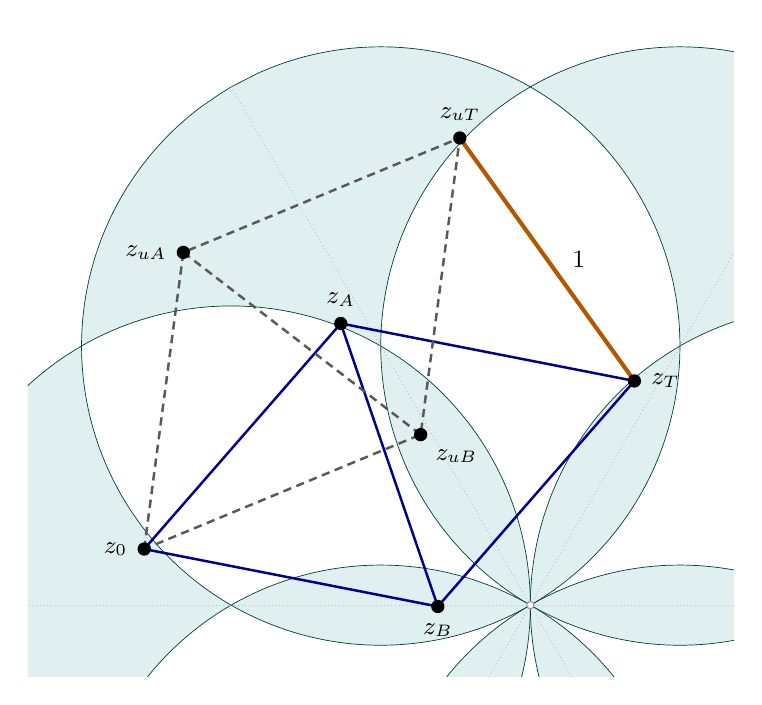
\begin{tikzpicture}[x=3.8cm,y=3.8cm,font=\small,
  vertex/.style={circle,fill=black,inner sep=1.7pt},
  first/.style={blue!55!black,line width=.9pt},
  second/.style={black!65,line width=.9pt,densely dashed}]
  \begin{scope}
    \clip (-1.68,-.24) rectangle (.68,1.93);
    \foreach \sector in {0,60,120,180,240,300} {
      \path[fill=teal!12,draw=teal!45!black,line width=.25pt]
        plot[domain=0:1,samples=101,variable=\r]
          ({\r*cos(\sector+acos(\r/2)-60)},
           {\r*sin(\sector+acos(\r/2)-60)})
        -- plot[domain=1:0,samples=101,variable=\r]
          ({\r*cos(\sector-acos(\r/2)+60)},
           {\r*sin(\sector-acos(\r/2)+60)}) -- cycle;
      \path[fill=teal!12,draw=teal!45!black,line width=.25pt]
        plot[domain=1:sqrt(3),samples=101,variable=\r]
          ({\r*cos(\sector+60-acos(\r/2))},
           {\r*sin(\sector+60-acos(\r/2))})
        -- plot[domain=sqrt(3):2,samples=101,variable=\r]
          ({\r*cos(\sector+acos(\r/2))},
           {\r*sin(\sector+acos(\r/2))})
        -- plot[domain=2:sqrt(3),samples=101,variable=\r]
          ({\r*cos(\sector-acos(\r/2))},
           {\r*sin(\sector-acos(\r/2))})
        -- plot[domain=sqrt(3):1,samples=101,variable=\r]
          ({\r*cos(\sector-60+acos(\r/2))},
           {\r*sin(\sector-60+acos(\r/2))}) -- cycle;
    }
    \foreach \sector in {0,60,120,180,240,300}
      \draw[black!25,densely dotted,line width=.35pt]
        (0,0) -- (\sector:2);
    \draw[fill=white,draw=black!45,line width=.3pt]
      (0,0) circle[radius=.012];
  \end{scope}
  \foreach \name/\gx/\gy in {
    O/0/0,
    A/{sqrt(3)/2}/{1/2},
    B/{sqrt(3)/2}/{-1/2},
    T/{sqrt(3)}/0,
    UA/{(5*sqrt(3)-sqrt(11))/12}/{(sqrt(33)+5)/12},
    UB/{(5*sqrt(3)+sqrt(11))/12}/{(sqrt(33)-5)/12},
    UT/{5*sqrt(3)/6}/{sqrt(33)/6}}
  {
    \coordinate (\name) at
      ({(35*(\gx-290/250)-12*(\gy+149/250))/37},
       {(12*(\gx-290/250)+35*(\gy+149/250))/37});
  }
  \draw[first] (O) -- (A) -- (T) -- (B) -- (O);
  \draw[first] (A) -- (B);
  \draw[second] (O) -- (UA) -- (UT) -- (UB) -- (O);
  \draw[second] (UA) -- (UB);
  \draw[orange!70!black,line width=1.5pt] (T) --
    node[midway,right=5pt,text=black] {$1$} (UT);

  \node[vertex,label=left:$z_0$] at (O) {};
  \node[vertex,label=above:$z_A$] at (A) {};
  \node[vertex,label=below:$z_B$] at (B) {};
  \node[vertex,label=right:$z_T$] at (T) {};
  \node[vertex,label=left:$z_{uA}$] at (UA) {};
  \node[vertex,label=below right:$z_{uB}$] at (UB) {};
  \node[vertex,label=above:$z_{uT}$] at (UT) {};
\end{tikzpicture}

\caption{The Moser graph in the placement $z_g$. All eleven drawn edges
have unit length. The two triangles sharing $z_Az_B$ force $z_0,z_T$
to have the same color in any proper three-coloring; the dashed diamond forces
$z_0,z_{uT}$ to have the same color. The highlighted edge $z_Tz_{uT}$
contradicts these equalities. The shading gives a cropped view of the open
region \eqref{eq:source-27}, using sampled analytic boundaries; the
boundaries and radii zero, one, and two are excluded. Dotted rays mark
the sector boundaries at multiples of \(\pi/3\).
The rational certificate in Section~\ref{sec:angular-certificate-verification}
proves strict membership of every vertex in that region, which is
restricted almost everywhere to three labels.}
\label{fig:moser-placement}
\end{figure}

The following certificate gives the strict membership needed to finish
the geometric argument.

\begin{lemma}[Seven-point certificate]\label{lem:angular-certificate}
Every \(z_g\) in \eqref{eq:angular-placement} satisfies
\(0<\abs{z_g}^2<4\) and \eqref{eq:source-27}.
\end{lemma}

The full rational verification is given in
Section~\ref{sec:angular-certificate-verification}.  We first use the
certificate to finish the geometric argument.

\begin{proposition}\label{prop:angular-three}
The extracted interface cycle cannot have length three.
\end{proposition}

\begin{proof}
Lemmas~\ref{lem:angular-region} and \ref{lem:angular-certificate}
give, for each of the seven points \(x+z_g\), an open
neighborhood restricted almost everywhere to the triangle
labels.  Choose \(\rho>0\) so that each point remains in
its corresponding neighborhood after any common translation
\(t\in B(0,\rho)\).  For each vertex, the translations
that put it outside the typical set, or in the null subset
where a nontriangle label occurs, form a null set.  The
union of these seven exceptional translation sets is null.
Choose \(t\) outside that union.  All seven translated
vertices are then typical and use the three triangle labels.
Their unit edges are preserved by the placement and common
translation, and typical-point properness gives a proper
three-coloring of the graph in
\eqref{eq:angular-seven-vectors}.  The two shared-edge
triangle pairs proved that this graph has no such coloring.
\end{proof}

\begin{proof}[Proof of Theorem~\ref{thm:weak-five}]
If a weak measurable five-coloring existed,
Proposition~\ref{prop:interface-cycle} would produce an
interface cycle of length three, four, or five with the
common-center and exclusion properties used above.
Propositions~\ref{prop:angular-five}, \ref{prop:angular-four},
and \ref{prop:angular-three} exclude all three possibilities.
Thus no weak measurable five-coloring exists.
\end{proof}

\subsection{Rational verification of the seven-point certificate}
\label{sec:angular-certificate-verification}

All terminating decimals in this verification denote exact rational
numbers.

\begin{proof}[Proof of Lemma~\ref{lem:angular-certificate}]
Table~\ref{tab:angular-coordinates} gives coordinate centers
\((\xi_0,\upsilon_0)\), each within \(h=0.00011\) of
the corresponding exact coordinate of \(z_g\), and strict
upper and lower polynomial bounds.
\begin{table}[htbp]
\centering
\begin{tabular}{@{}crrrr@{}}
\toprule
\(g\)&\(\xi_0\)&\(\upsilon_0\)&\(P_+\)&\(P'_-\)\\
\midrule
\(0\)&\(-1.2906\)&\(0.1876\)&\(0.90\)&\(1.35\)\\
\(A\)&\(-0.6335\)&\(0.9414\)&\(0.095\)&\(0.110\)\\
\(B\)&\(-0.3092\)&\(-0.0045\)&\(0.000002\)&\(0.00065\)\\
\(T\)&\(0.3478\)&\(0.7493\)&\(0.023\)&\(0.026\)\\
\(uA\)&\(-1.1598\)&\(1.1790\)&\(9.8\)&\(19.0\)\\
\(uB\)&\(-0.3666\)&\(0.5700\)&\(0.0022\)&\(0.024\)\\
\(uT\)&\(-0.2358\)&\(1.5614\)&\(12.65\)&\(12.9\)\\
\bottomrule
\end{tabular}
\caption{Coordinate boxes and bounds \(P<P_+<P'_-<P'\).}
\label{tab:angular-coordinates}
\end{table}

Here are explicit checks of the boxes and polynomial bounds.
Squaring rational endpoints proves
\[
 1.73205<\sqrt3<1.73206,\qquad
 3.31662<\sqrt{11}<3.31663.
\]
Put \(a_*=1.732055\), \(b_*=3.316625\), and
\(\epsilon=0.000005\).  Replacing the two radicals by
these midpoints changes their product by less than
\[
 (a_*+b_*)\epsilon+\epsilon^2
 =0.000025243425<0.000026.
\]
The coordinates of the three products in
\eqref{eq:angular-seven-vectors} are
\begin{align*}
 uA&=\left(\frac{5\sqrt3-\sqrt{11}}{12},
                 \frac{\sqrt{33}+5}{12}\right),\\
 uB&=\left(\frac{5\sqrt3+\sqrt{11}}{12},
                 \frac{\sqrt{33}-5}{12}\right),\\
 uT&=\left(\frac{5\sqrt3}{6},\frac{\sqrt{33}}6\right).
\end{align*}
For each coordinate of every \(g\), the midpoint substitution
therefore has error at most \(\epsilon\): the largest product
error is less than \(0.000026/6<\epsilon\), and the other
coefficients give this bound directly.  The rotation in
\eqref{eq:angular-placement} has absolute row sum \(47/37\).
For an exact check of the displayed centers, let
\(\widetilde z_g\) denote the placed point after this rational
midpoint substitution.  Direct substitution gives the residuals
\[
 \widetilde z_g-(\xi_0+i\upsilon_0)
       =\frac{d_x+i d_y}{710400000000},
 \qquad
 \begin{array}{c|rr}
 g&d_x&d_y\\\hline
 0&3840000&-23040000\\
 A&-29520000&10176000\\
 B&-12240000&-22464000\\
 T&25440000&10752000\\
 uA&32043244&-19212795\\
 uB&4763244&-27212795\\
 uT&32966488&-23385590
 \end{array}
\]
Every residual numerator has magnitude less than
\(35520000=710400000000/20000\), proving that the midpoint-substituted coordinates
have the stated four-decimal roundings, with error less than
\(0.00005\).  Thus every final coordinate error is bounded by
\[
 \frac{47}{37}\epsilon+0.00005<0.00011=h.
\]

For completeness, the remaining interval calculations reduce
to the small rational factors in Table~\ref{tab:angular-factors}.
Define
\begin{align*}
 x_l&=(\abs{\xi_0}-h)^2,&x_u&=(\abs{\xi_0}+h)^2,\\
 y_l&=(\abs{\upsilon_0}-h)^2,&y_u&=(\abs{\upsilon_0}+h)^2,\\
 l_l&=x_l+y_l,&l_u&=x_u+y_u,\\
 H&=\max(\abs{3x_l-y_u},\abs{3x_u-y_l}).
\end{align*}
All listed absolute coordinate centers exceed \(h\), so
these intervals enclose \(\xi^2,\upsilon^2,l\).
In each row the factors in the second table satisfy
\[
 y_u<b_y,\qquad H<b_H,\qquad a<l_l\le l_u<b.
\]
These claims require only squaring integers: with
\(M=10^5\), \(m=M\abs{\xi_0}\), \(n=M\abs{\upsilon_0}\),
the four squared-coordinate endpoints are
\[
 (x_l,x_u,y_l,y_u)
 =\frac1{10^{10}}
   \bigl((m-11)^2,(m+11)^2,(n-11)^2,(n+11)^2\bigr).
\]
Thus every entry is verifiable using the displayed coordinate
integers, without evaluation of an irrational number.
\begin{table}[htbp]
\centering
\begin{tabular}{@{}crrrr@{}}
\toprule
\(g\)&\(b_y\)&\(b_H\)&\(a\)&\(b\)\\
\midrule
\(0\)&\(0.0353\)&\(4.963\)&\(1.70\)&\(1.71\)\\
\(A\)&\(0.887\)&\(0.319\)&\(1.28\)&\(1.29\)\\
\(B\)&\(0.000022\)&\(0.287\)&\(0.095\)&\(0.096\)\\
\(T\)&\(0.562\)&\(0.199\)&\(0.682\)&\(0.683\)\\
\(uA\)&\(1.391\)&\(2.647\)&\(2.73\)&\(2.74\)\\
\(uB\)&\(0.326\)&\(0.079\)&\(0.459\)&\(0.46\)\\
\(uT\)&\(2.44\)&\(2.273\)&\(2.493\)&\(2.495\)\\
\bottomrule
\end{tabular}
\caption{Rational factors bounding the squared-coordinate boxes.}
\label{tab:angular-factors}
\end{table}

Every interval \((a,b)\) lies in \((0,4)\) and avoids one.
The polynomial factors are therefore bounded by
\begin{align*}
 P&\le y_u H^2<b_yb_H^2<P_+,\\
 P'&\ge l_l^3(1-l_u/4)
          \min(\abs{l_l-1},\abs{l_u-1})^2\\
   &>a^3(1-b/4)\min(\abs{a-1},\abs{b-1})^2>P'_-.
\end{align*}
The last inequalities are direct rational products of
the second table, with the target bounds in the first.
For example, its final row gives
\[
 2.44(2.273)^2<12.65,
 \qquad
 (2.493)^3(1-2.495/4)(1.493)^2>12.9.
\]
The other six rows give the corresponding displayed strict
bounds by the same two products.  The squared-radius
intervals also lie respectively in
\[
 (1.70,1.71),\ (1.28,1.29),\ (0.095,0.096),\ (0.68,0.69),
 \ (2.73,2.74),\ (0.459,0.46),\ (2.49,2.50).
\]
Finally \(P_+<P'_-\) in every row of
Table~\ref{tab:angular-coordinates}.  This proves
\eqref{eq:source-27} and the radius conditions for all seven
vertices.
\end{proof}
